% chapitre de description du travail technique
\chapter{Technical work}

\label{technic}

%-------------------
% Define some commands to keep the formatting separated from the content
\newcommand{\keyword}[1]{\textbf{#1}}
\newcommand{\tabhead}[1]{\textbf{#1}}
\newcommand{\code}[1]{\texttt{#1}}
\newcommand{\file}[1]{\texttt{\bfseries#1}}
\newcommand{\option}[1]{\texttt{\itshape#1}}

%---------------------

\section{Code Refactoring}
When working with new code, the first thing to do is to understand it. Then, you have to do the necessary modifications.
\subsection{Understanding the code}
When I arrived at IRI, Another student was already working on applying particle filtering on a robot simulation.

When first discovered, the code was mainly organized in three parts :
\begin{itemize}
  \item The Interval class
  \item The Box particle filtering
  \item The Main
\end{itemize}
\subsubsection{The Interval Class}
The interval class was directly inspired by Mr Jaulin's works and courses \parencite{IAMOOC}.
It's a simple class enabling the use of Interval analysis in Matlab, by creating a new object, and overloading the standard comparators and operators.

As such, this new object is in fact defined by a couple upper bound and lower bound for each dimension we are in.
In this case, the simulation we work on is two dimensional, so the intervals have two bounds of each kind.
\subsubsection{The Box particle filtering}
"Resulting from the synergy between the sequential Monte Carlo method and interval analysis, box particle filtering is an approach that has recently emerged and is aimed at solving a general class of nonlinear filtering problems.
This approach is particularly appealing in practical situations involving imprecise stochastic measurements that result in very broad posterior densities.

It relies on the concept of a box particle that occupies a small and controllable rectangular region having a nonzero volume in the state space.
Key advantages of the box particle filter against the standard particle filter are its reduced computational complexity and its suitability for distributed filtering.

Indeed, in some applications where the sampling importance resampling PF may require thousands of particles to achieve accurate and reliable performance, the box-PF can reach the same level of accuracy with just a few dozen box particles."\parencite{BPF}

As seen, the BPF is an efficient system of filtering
\subsubsection{The Main}
Two more files are used in the program.

In the environement file, all the variables needed at the start of the program,
 such as the trajectory, the number of boxes, or the length of the simulation are defined.

The Mainbox file is simply the main loop, and the one where the graphical interface is created. It's no more than printing the trajectories for the real and the self-percieved bots.

\subsection{Changing the way it works}
The first thing to do was to change completely how the main loop worked.
the new system needed to be robust, simple and calculate step after step.

\begin{figure}[th]
\centering
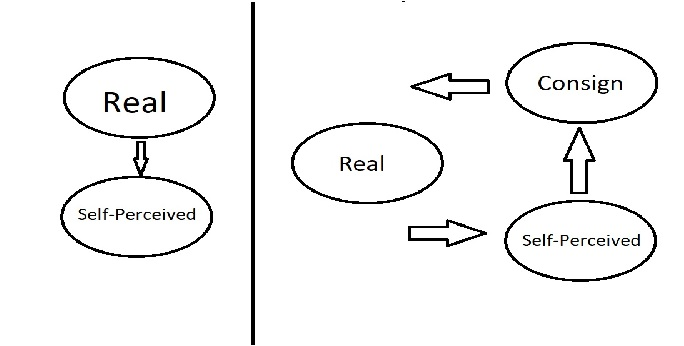
\includegraphics{Figures/Loops}
\decoRule
\caption[the new loop]{How the new control loop was implemented.}
\label{fig:Loops}
\end{figure}

In the first program, the point of interest was measuring the position and the speed of the robot.
The system had no feedback loop, so there was no need to calculate step by step. All the calculation for the robot's position and movement were done before the program's actual work began.
The new feedback loop needed all the parameters from a step to calculate the next one.

Informations from the consign trajectory and the self-perceived robot were used to calculate the real position of the robot.
The real position was then used to infer the new self-perceived position, feeding the loop again.

From one point to another, the system had many calculations to do, primarily due to the BPF.
Indeed, the BPF is a system which needs a lot of diverse points to operate efficiently. A sample size of 2000 points was sometimes reached.
My feedback loop and control system needed to be light and fast, or it would have slowed the program even more.


\section{Simple control}
After the new loop was added, I had to modify the informations sent from one part of the loop to another.

\subsection{Adding precision}
Before the work on control algorithm started, I had discovered that the informations returned by the BPF were much more precise than simply using the sensor's feed, but consistency was lacking.
Indeed, from one step to another, the BPF could render highly different results, and it would cause the real robot behaving eratically.
To compensate, a low-pass filter was added, by using a sliding median of the last five values instead of only the last one.

Although such a system means that the correction is a bit late, it suppresses most of the eratical behavior from the self-perceived bot.
Giving more weigth to the last value was tested, but the eratical behavior came back with too much force, so the idea was droped.
More tests were made with a sliding median on more or less values, but five was the best compromise.
The system was only around two steps late, so about 1/10th of a second.

\subsection{Testing methods and taking control}

The new loop, at the begining, did nothing more than transmitting informations from one part of the program to another.
At first, a simple proportional control was added. A divergence from the original trajectory was met by a correction proportional to the deviation.

This system was too unstable or too slow.
As it is often the case for proportionnal control, the bot would either overshoot, or not be able to reach the deignated trajectory.

The next step was using a proportionnal derivative method. This solved the overshoot problems I had, and the corrections were much faster.
It was implemented in a simple way, by adding a control variable named U.
%code?

I then tried to adapt a H-infinity control method, but a few problems blocked my way.
The more evident one was that the model I used was far from enough for this method to yield good results.
And of course, the use of a BPF resulted sometimes in singularities or in a kind of saturation that rendered the method completely unusable.


\section{Obstacle Avoidance}
Now that the robot was able to follow a trajectory, with more or less success, depending on the precision reached by the BPF, it needed to avoid obstacles and walls.


\subsection{Trials and errors}

One of the best ways to avoid obstacles in a partially known environement is a vector field.
In my case, I had to add the right vector to the vector I had already created with the control system.

My first try was simply by adding repulsive vectors stemming from boxes colliding with a wall.
This test was far from successfull, since the self-perceived robot, a bit late because of the low-pass filter, would often make a U-turn, and completely lose itself.
Indeed, the vector field, radiating only from colliding boxes, would overrun the control vector and push back the robot until the robot was far enougth from the consign for shenanigans to ensue.


\subsection{Creating a vector field}

I had to devise a way for the robot to be aware of his suroundings as a whole.
 I then created a small sub program able to infer a repulsive vector field from an image of the obstacles.

 % way of creating and images

\section{Graphic User Interface}

Since my work was a bit tedious on someting so dry, I decided to add a graphical interface.

\subsection{Adding an interface}

\subsection{Preparing for later}
